\chapter{Miscellaneous Bits of Code}
\label{sympy6jAppendix}

\section{Calculation of Dipole Moment Operator}
This calculation is relatively straightforward. However, when dealing with a lot of constants, it is easy to use an online service to keep things straight. For this calculation, I prefer to enter ``sqrt(3*hbar*c\^3/(4*(2*pi*c/407.771 nm)\^3)*4*pi*epsilon\_0*4*1.41e8*1/s)'' as a query into Wolfram Alpha. The result (as of 2015-11-25) can be found 
\href{http://www.wolframalpha.com/input/?i=sqrt%283*hbar*c%5E3%2F%284*%282*pi*c%2F407.771+nm%29%5E3%29*4*pi*epsilon_0*4*1.41e8*1%2Fs%29}{here}.
The result turns out to be 4.344 Bohr dipole moments.
\section{Hyperfine splitting}
This is a Jupyter notebook containing Python 2 code to calculate the hyperfine splitting.
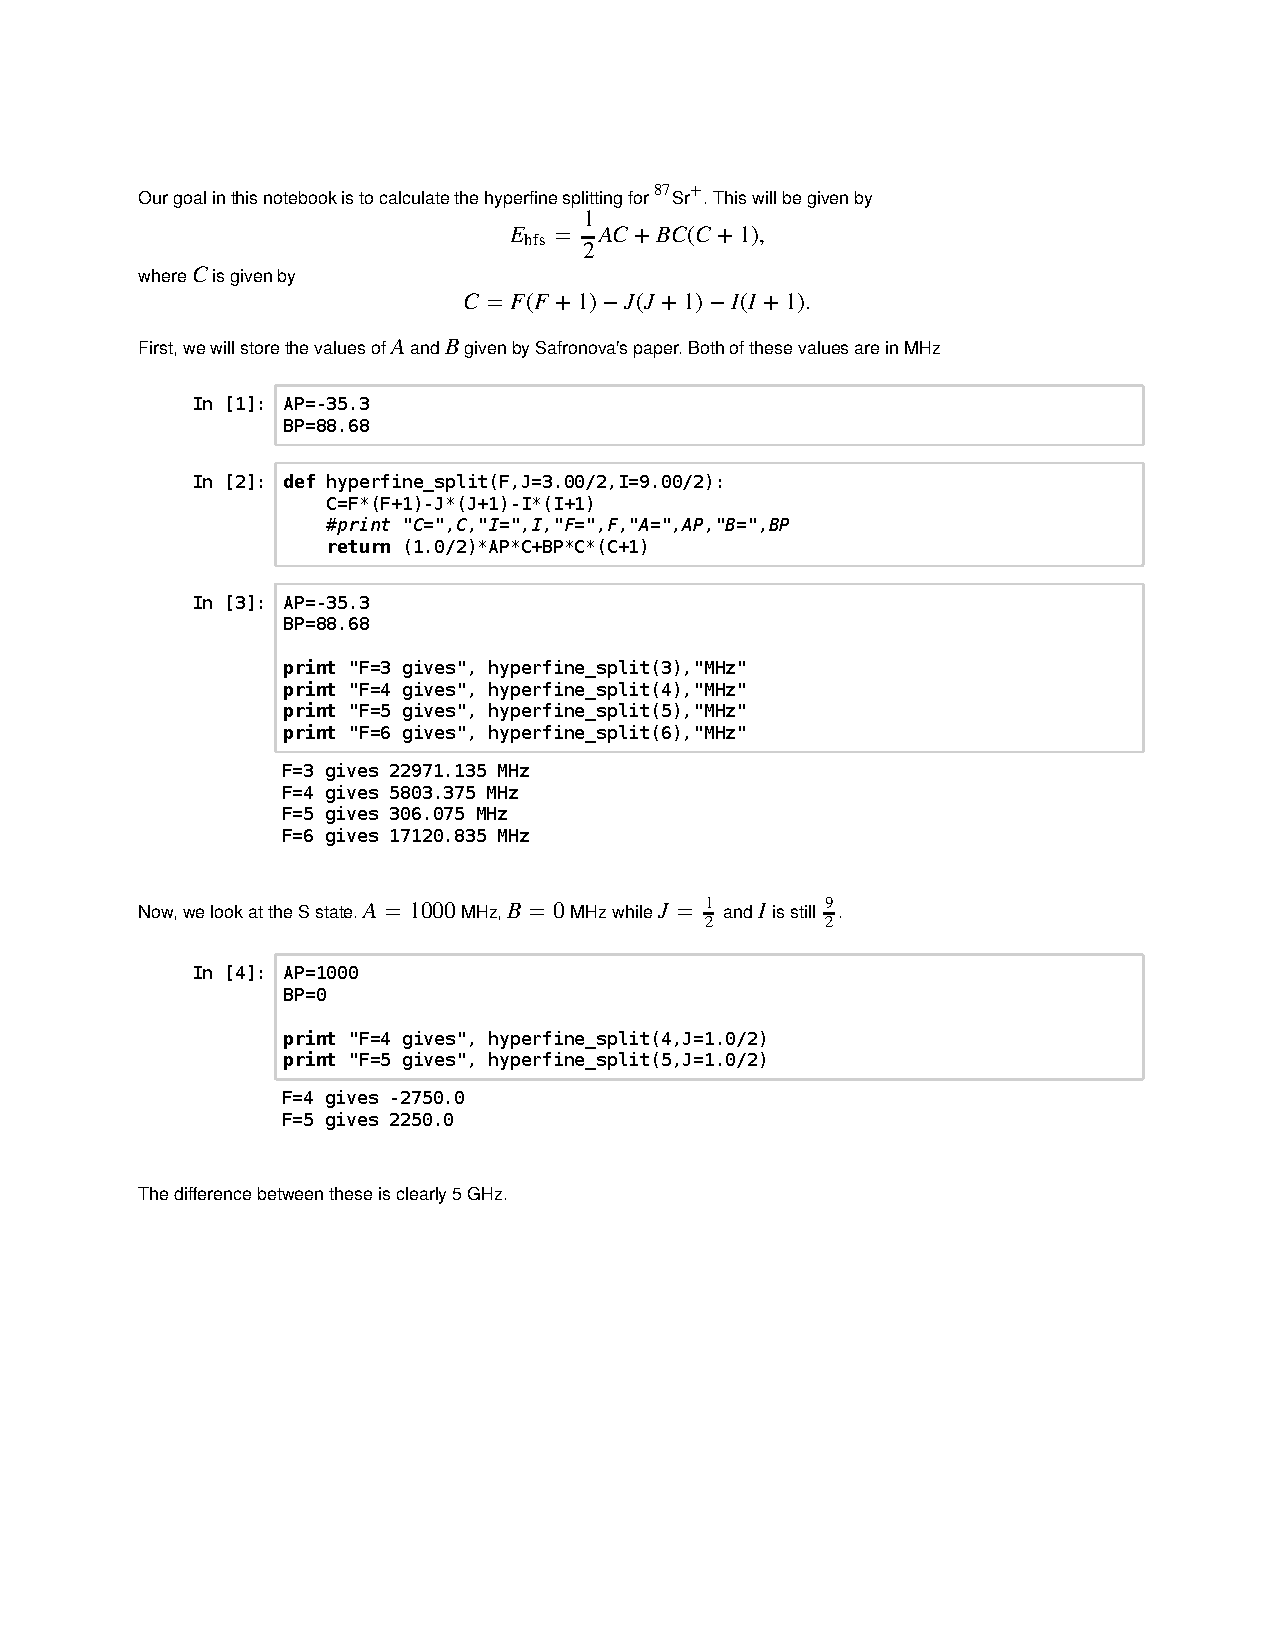
\includepdf[pages={1-2}]{hyperfine_splitting2}
\section{Clebsch-Gordan coefficient calculation}
When using the Wigner-Eckhart theorem in Chapter\,\ref{ChapterAboutTheAtoms}, I used this code to calculate the coefficients. I was not sure which states could be viably identified as $|i\rangle$, $|e\rangle$ and $|g\rangle$, so I somewhat used brute force to see which Clebsch-Gordan coefficients turned out to be nonzero. 
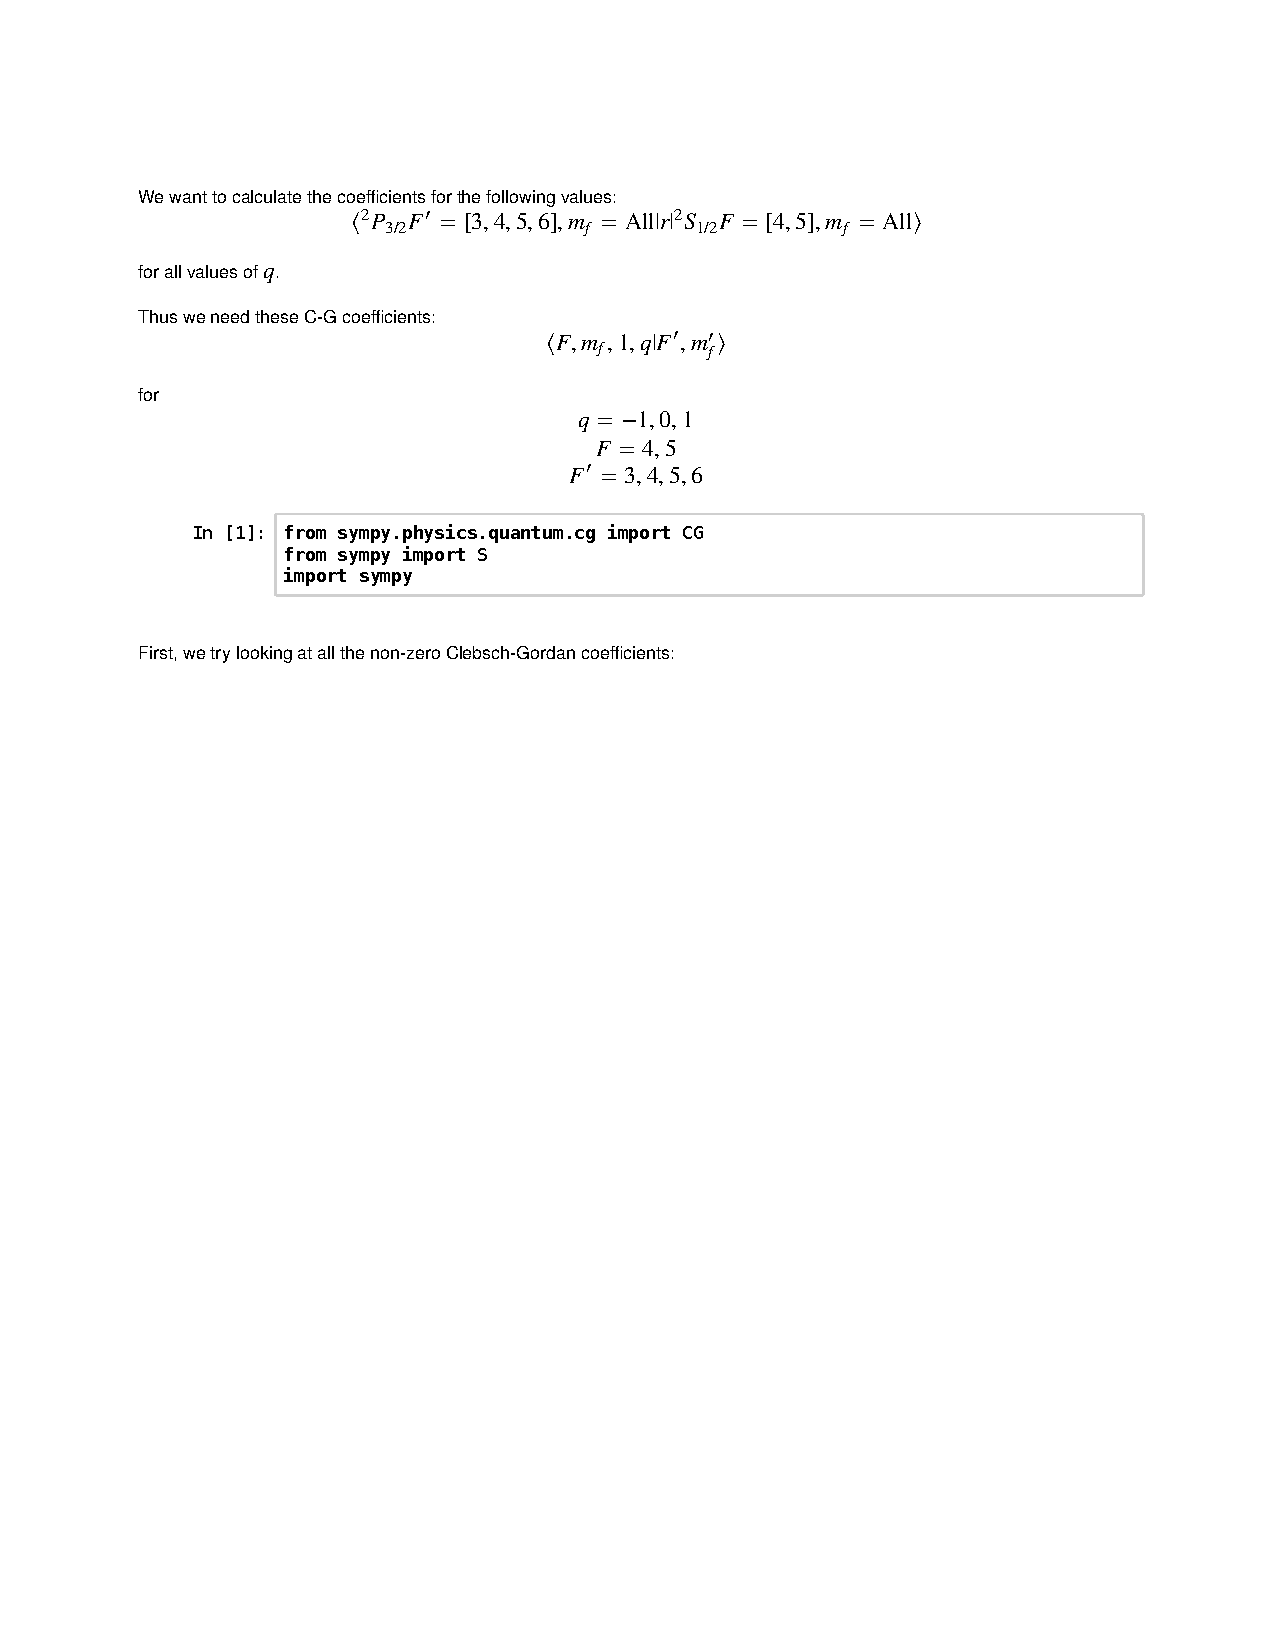
\includepdf[pages={1-4}]{CGcoefficients2}
\section{Spectator theorem}
In Chapter\,\ref{ChapterAboutTheAtoms}, we had a need to look up the Wigner 6j symbols for various states. This was done using the following code:
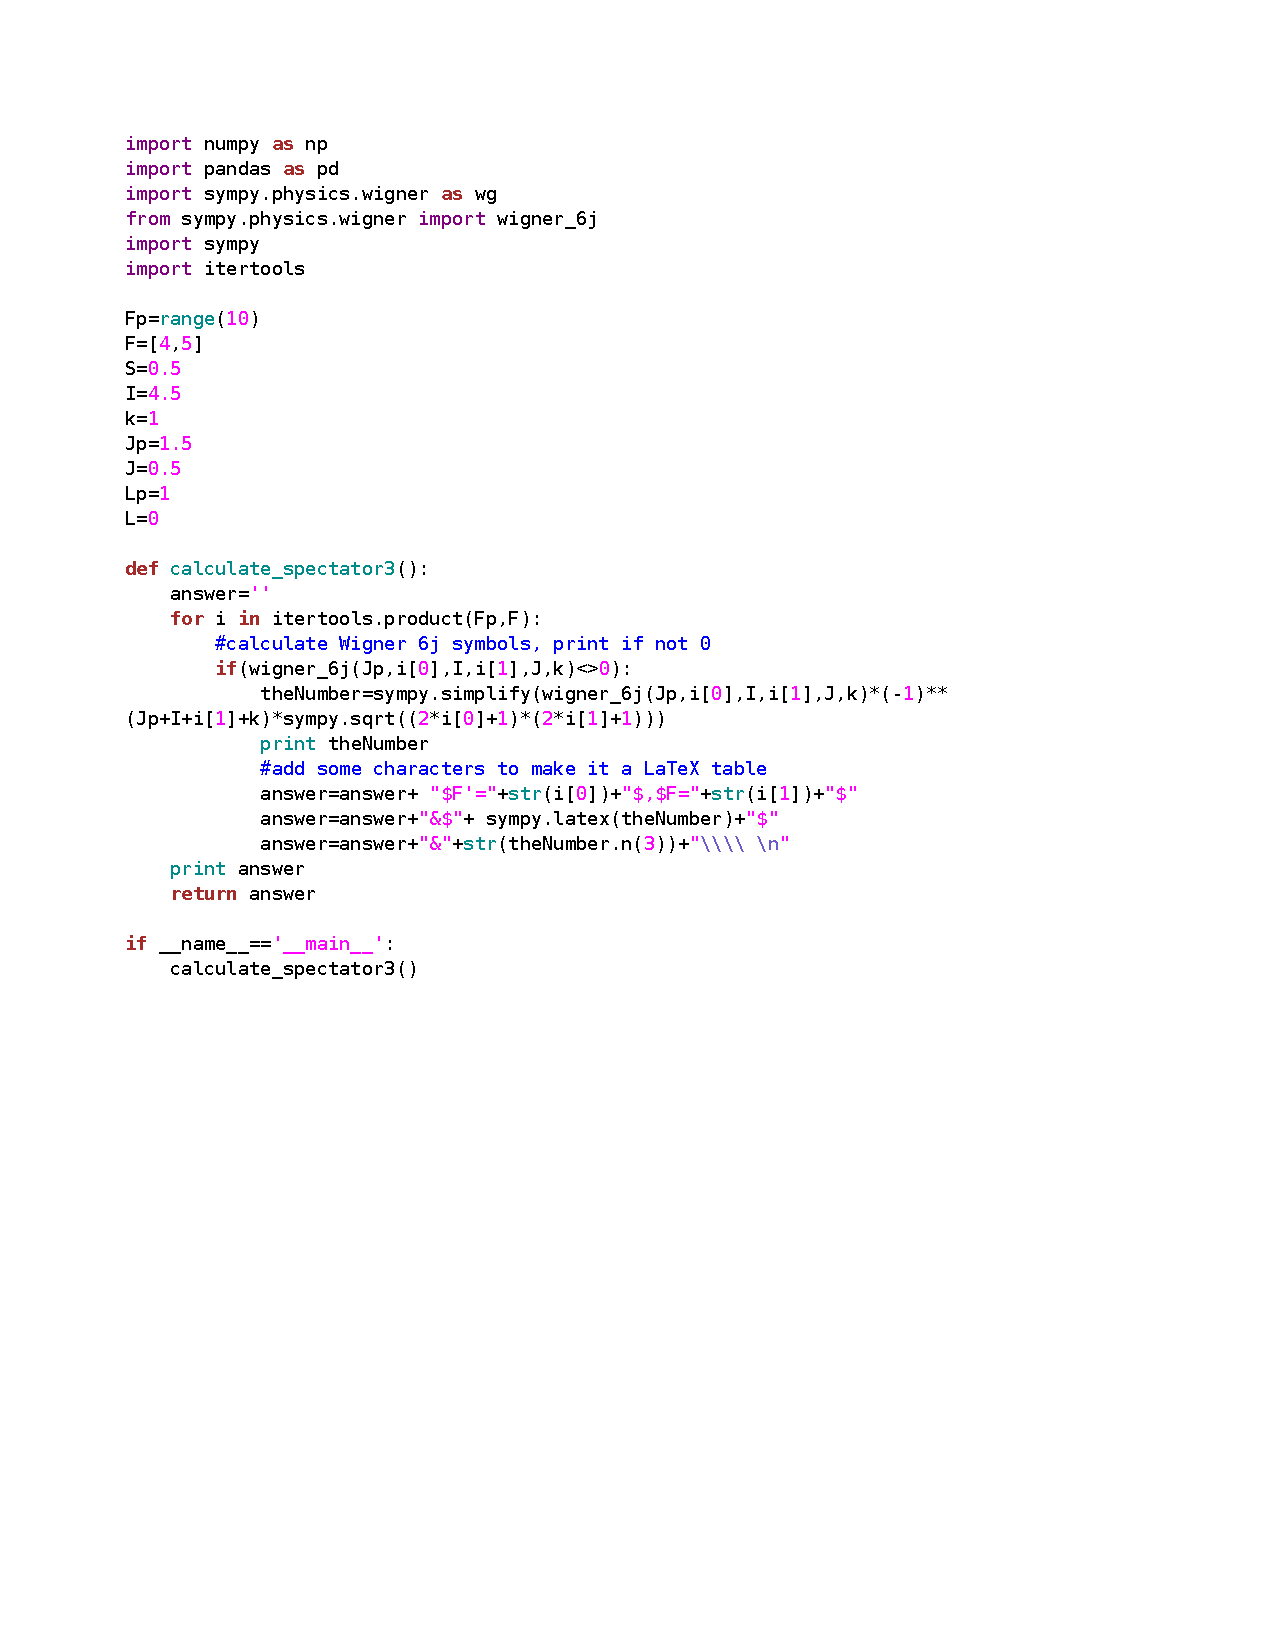
\includepdf[pages={1-1}]{spectator_theorem}
